
\section{Evaluation} \label{sec:evaluation}
We conducted extensive simulations to justify the improvement over the three key metrics we defined in \autoref{subsec:metrics}. The setup and baseline algorithms is in \autoref{sub:setup}. We show the improvement space in \autoref{sub:oracle} where the estimated bandwidth is from an oracle prediction and show our algorithm performs close-to-optimal in a noisy prediction scenario in \autoref{sub:noisy}. 

\subsection{Setup} \label{sub:setup}
 The available bandwidth traces are taken from one major U.S. 4G network carrier and MIT Sprout Project\cite{Sprout}. We cut wireless channel traces into 5-10 minutes long segments, as 80-90\% video sessions are shorter than 10 mins\cite{ATTVIDEO}. In total there are four 3G and 12 4G segments. We take 10 different video encoding rates from one major video streaming carrier: $\{0.235,0.375, 0.56\dots4.3\}$ Mbps \cite{NETFLIXRATE} and we assume no variation in bit rates for each chunk. 

We choose two different streaming algorithms for comparison; FESTIVE \cite{Festive} and BBA \cite{BBA}. We first choose FESTIVE because the algorithm is designed for the scenario where there are several users sharing a single bottleneck link during video streaming session, which fits the cellular network setting where the wireless channel is the bottleneck. It takes the harmonic mean of bandwidth over the last 20 video chunk downloads as reference and adds randomization into video chunk download scheduling to avoid a synchronized congestion. BBA class algorithms are designed to avoid interruption and rebuffering, and it can sustain up to tens of seconds connection loss. It relies on video buffer occupancy as an implicit feedback of the network condition for video bit rate selection, and use a linear relation to the buffer occupancy to compute the desired rate. It also has a fast startup phase where it ramps up to a desirable play bit rate based on buffer occupancy growth rate. Throughout our experiments, for FESTIVE we set the tunable knob for stability $\alpha =12 $, bandwidth factor $p=1$ and recommended buffer size 60 seconds. In BBA we are using BBA(2) with $BufferReservior=90s$, $BufferCushion=126s$ and max buffer $z=240s$. In our approach we set risky phase $B_risk=60s$ and max buffer $z=240s$, look back chunk size $k=5$ and $\alpha=0.15$. Each video chunk is 4 seconds, which is a prevalent length for one major video streaming vendor. 



%\subsection{Algorithm Performance}



\begin{figure}[t]
 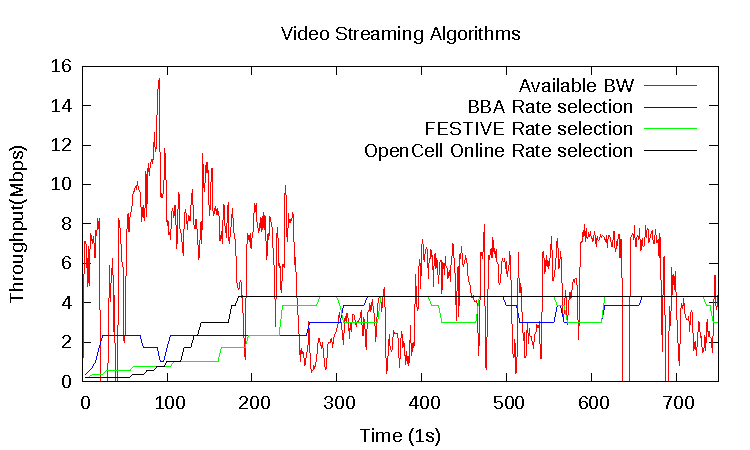
\includegraphics[width=\linewidth]{pictures/ATT.pdf}
 \caption{A sample trace from one major 4G network}
\end{figure}

\begin{table}[t]

\begin{tabular} {|c |c |c |c |}
\hline
\textbf{ Improvement} &\textbf{Quality} &\textbf{Stability} & \textbf{Interruption}\\ \hline
BBA(3G)  & 1.16x& 2.87x& 1x \\ \hline
FESTIVE(3G)    & 1.39x & \textcolor{red}{0.68x}&2.5x\\ \hline
BBA(4G) & 1.15x&3.8x& 1x* \\ \hline
FESTIVE(4G) & 1.32x& 3.6x& 1x* \\ \hline
\end{tabular}
\centering
\caption{\large Improvement with oracle estimator\newline \small*no interruption occurred during play} \label{cap:table}
\end{table}



\subsection{Oracle Estimator}\label{sub:oracle}
In this section, the algorithm is using an "oracle" estimator, to show the space of improvement.

\emph{Key metrics improvement:} we measure three different metrics: quality (play efficiency), stability and interrupts. Our algorithm outperforms the other two algorithms in all traces in terms of all three metrics except for stability in two 3G trace comparing to FESTIVE, and the summary is in \autoref{cap:table}. For the traces where FESTIVE achieves higher stability, FESTIVE tends to stay at low play bit rates and thus has much lower quality and link utilization, we also note in these traces the stability issue is less important: our algorithm has 5.5 switches on average while FESTIVE has 3 switches, and in all other traces all algorithms have $>$6 switches. 
\begin{figure}[t]
\centering
 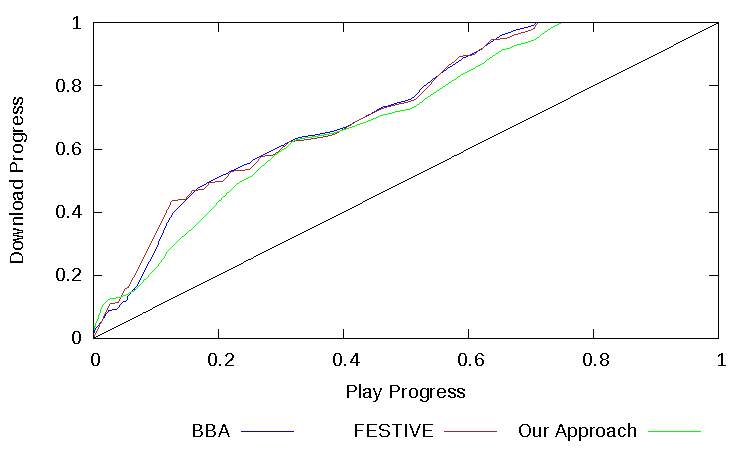
\includegraphics[width=\linewidth]{pictures/ATT_downloading.pdf}
 \caption{Buffer Prefetching} \label{fig:download}
\end{figure}
%\emph{Key metrics improvement:} we measure four different metrics: quality (play efficiency), stability and interrupts. Link utilization measures the total download vs available bandwidth, and the value is one if the link is constantly saturated. Play efficiency measures during the play session, the video downloaded and played vs available bandwidth, in the case without prefetched chunks, download utilization and play efficiency are equal. Stability measures the number of bit rate switches and interrupts measures the occurrence of interruption. Our algorithm outperforms the other two algorithms in all traces in terms of all four metrics, and the summary is in \autoref{cap:table}.

\emph{Prefetched buffer size}: we also compare the prefetched buffer size between BBA and our approach. FESTIVE is not client video buffer based solution and only adds randomized scheduling if it reaches a certain buffer level, we extend that buffer level to $z=240s$ download and see no difference in terms of FESTIVE's efficiency, stability or interruption, since FESTIVE only looks at past 20 chunks. Comparing BBA, we have reduced buffer size significantly by 10-40 seconds even though both maximum buffer sizes $z=240$. One sample trace is in \autoref{fig:download}: ideally the download progress and play progress are on the red line, however due to prefetching the download time is always ahead of play time, or the download line is always above the red line and the gap is the client play buffer size.

\begin{table}[t]
\small
\begin{tabular} {|c|c|c|c|}
\hline
 &\textbf{BBA} &\textbf{FESTIVE} &\textbf{Our Approach} \\ \hline
Ramp-up Time& 560s& 260s& 144s\\ \hline\hline
Link Loss(30s)& 1.05 Mbps& 1.05 Mbps& 4.3 Mbps\\ \hline
Link Loss(45s)& 1.05 Mbps& 1.05 Mbps&1.05 Mbps\\ \hline
Link Loss(60s)& 0.235 Mbps& 1.05 Mbps&1.05 Mbps\\ \hline
\end{tabular}
\centering
\caption{Ramp-up time and resilience to link outage} \label{cap:table2}
\end{table}

\emph{Fast ramp up and resilience to connection loss:} we use a synthetic trace to test the algorithms' properties. We set the bandwidth to static at 4.3 Mbps to test ramp-up time. We also add 30, 45 and 60 seconds connection outage after 100 seconds 4.3 Mbps bandwidth to test the resilience of the algorithm. All algorithm encounters zero interruption in all cases, our algorithm and FESTIVE's play bit rates are 4.3 Mbps at the moment, while BBA's is 1.75 Mbps. (Note the difference between play time and download time, FESTIVE takes 260s play time to get to 4.3 Mbps, but at 100s download time FESTIVE is downloading video chunk at bit rate 4.3 Mbps, the gap is due to prefetching) Algorithms suffer from dropping to a lower quality, and the new low quality values are summarized in \autoref{cap:table2}. This shows our algorithm has a good performance margin in both ramp-up time and resilience to link loss. 



\emph{Comparison with Theoretical Max Quality}: for a formulation in \autoref{subsec:offline}, we use IBM CPLEX to solve the mixed integer problem. We again replayed the 16 traces and the result shows that our approach can achieve 84\% of the efficiency upper bound. For the formulation in \autoref{subsec:offline} one 3G trace has no feasible solution, and the reason is from the zero-interruption constraint, which also justifies the inevitability of interruption occurred in online algorithms. 

%\emph{Comparison with Modified FESTIVE}\Note{Not done yet!}: to show the performance gain is from both the novel algorithm and exposed extra KPIs, we also modified FESTIVE: we feed FESTIVE with a future bandwidth instead of using its harmonic mean estimation. 

\begin{comment}
\begin{table}[t]

\begin{tabular} {|c |c |c |c |}
\hline
 Improvement &Quality &Stability & Interruption\\ \hline
BBA(3G)  & 1.16x&1.6x &\textcolor{red}{0.9x} \\ \hline
FESTIVE(3G)& 1.40x &\textcolor{red}{0.86x}& 5x\\ \hline
BBA(4G) & 1.17x& 1.9x& N/A \\ \hline
FESTIVE(4G) & 1.14x& 3.4x& N/A \\ \hline
\end{tabular}
\centering
\caption{Improvement with noisy estimator} \label{cap:table2}
\end{table}
\end{comment}
\subsection{Noisy Estimator}\label{sub:noisy}
We use a synthetic estimator for prediction and show that when the prediction is roughly accurate with a certain degree of error rate, our algorithm is robust to achieve a close-to-optimal performance. We conduct a sensitive study for the new algorithm with the noisy estimator. The synthetic estimator uses a noisy factor with a distribution of Gauss(1,0.2) or Uniform(0.5, 1.5) when offering predicted bandwidth. Through repetitive replay, we found the algorithm achieves about the same performance in all traces, but with around 10\% chance we have significant degradation in stability (1.5x quality switches) in the repetitive replay. 

